\documentclass[border=4pt]{standalone}
\usepackage{tikz}
\usepackage{amsmath,amssymb}
\usepackage{mathptmx}
\usetikzlibrary{arrows.meta,positioning,calc,shapes.geometric,decorations.pathreplacing,shadows,fadings,patterns}
\definecolor{cblue}{HTML}{1F4E9C}
\definecolor{cgold}{HTML}{D08C00}
\definecolor{cred}{HTML}{B5172E}
\definecolor{cgreen}{HTML}{1B7A3A}
\definecolor{cgrey}{HTML}{555555}
\definecolor{cpurple}{HTML}{5B2A86}
% oblique 3D cuboid: \cuboid{x}{y}{z}{dx}{dy}{dz}{colour}
\newcommand{\cuboid}[7]{%
  \fill[#7!55!white,draw=#7!60!black,line width=0.4pt] (#1,#2,#3+#6) -- ++(#4,0,0) -- ++(0,#5,0) -- ++(-#4,0,0) -- cycle;
  \fill[#7!80!black,draw=#7!60!black,line width=0.4pt] (#1+#4,#2,#3) -- ++(0,#5,0) -- ++(0,0,#6) -- ++(0,-#5,0) -- cycle;
  \fill[#7,draw=#7!60!black,line width=0.4pt] (#1,#2,#3) -- ++(#4,0,0) -- ++(0,0,#6) -- ++(-#4,0,0) -- cycle;}

\begin{document}
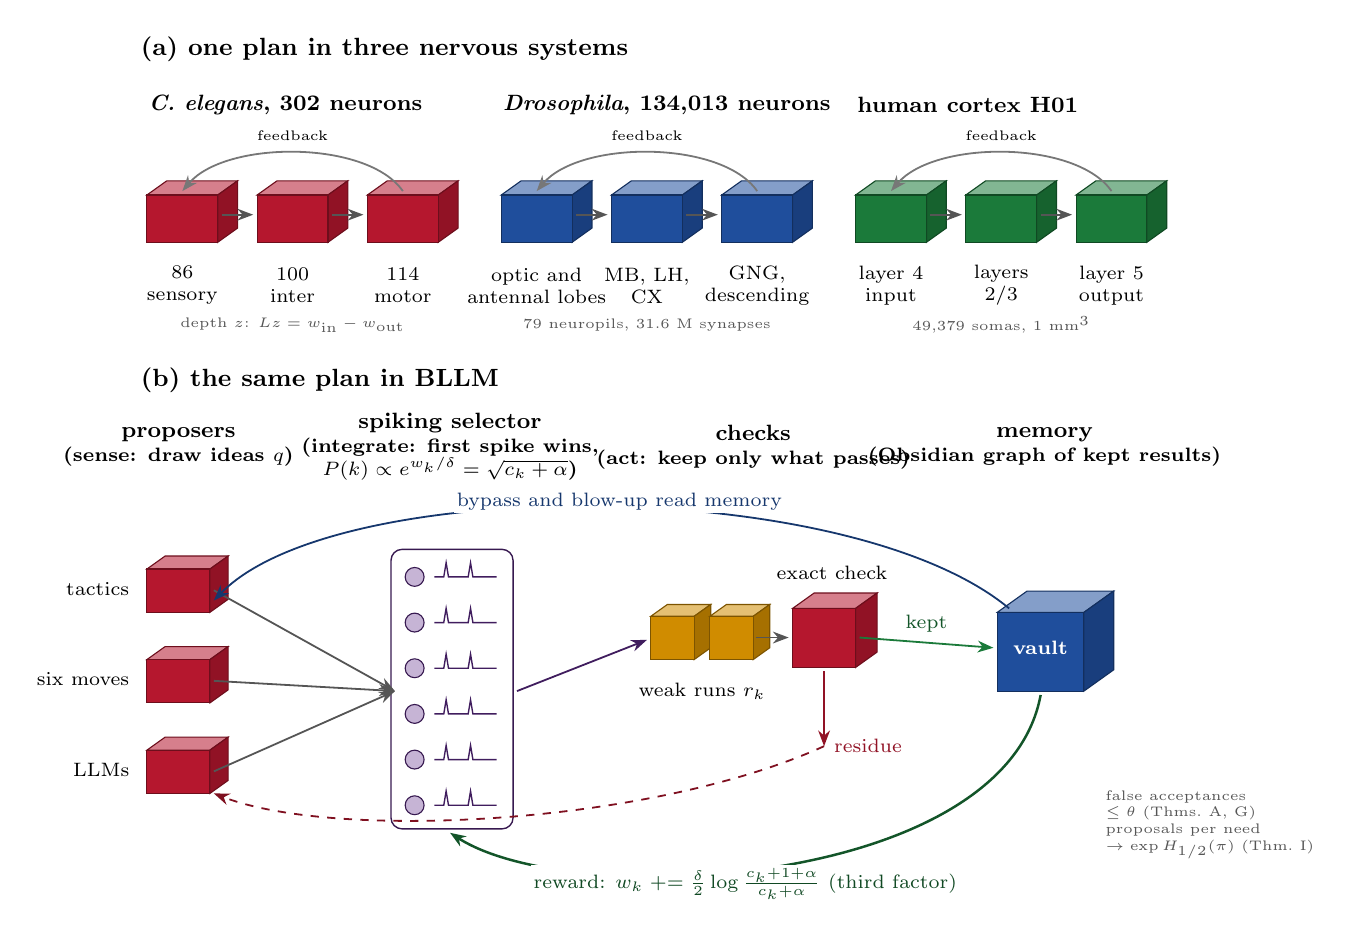
\begin{tikzpicture}[x={(1cm,0cm)},y={(0.42cm,0.3cm)},z={(0cm,1cm)},
  arr/.style={-{Stealth[length=2.0mm]},line width=0.65pt},
  lab/.style={font=\scriptsize,align=center},
  hd/.style={font=\footnotesize\bfseries,align=center},
  neu/.style={circle,draw=#1!60!black,fill=#1!35,inner sep=0pt,minimum size=2.4mm},
  spk/.style={line width=0.5pt,#1}]
% ---------------- row 1: the three animals, sense -> integrate -> act ----------------
\node[font=\small\bfseries,anchor=west] at (-0.6,0,10.05) {(a) one plan in three nervous systems};
\foreach \col/\name/\a/\b/\c/\note [count=\i from 0] in {
   cred/{\textit{C.\ elegans}, 302 neurons}/{86\\sensory}/{100\\inter}/{114\\motor}/{depth $z$: $Lz=w_{\mathrm{in}}-w_{\mathrm{out}}$},
   cblue/{\textit{Drosophila}, 134{,}013 neurons}/{optic and\\antennal lobes}/{MB, LH,\\CX}/{GNG,\\descending}/{79 neuropils, 31.6 M synapses},
   cgreen/{human cortex H01}/{layer 4\\input}/{layers\\2/3}/{layer 5\\output}/{49{,}379 somas, 1 mm$^3$}}{
  \pgfmathsetmacro\x{4.5*\i}
  \node[hd,anchor=west] at (\x-0.5,0,9.35) {\name};
  \cuboid{\x-0.4}{0}{7.6}{0.9}{0.6}{0.6}{\col}
  \cuboid{\x+1.0}{0}{7.6}{0.9}{0.6}{0.6}{\col}
  \cuboid{\x+2.4}{0}{7.6}{0.9}{0.6}{0.6}{\col}
  \node[lab] at (\x+0.05,0,7.05) {\a};
  \node[lab] at (\x+1.45,0,7.05) {\b};
  \node[lab] at (\x+2.85,0,7.05) {\c};
  \draw[arr,cgrey] (\x+0.55,0,7.95) -- (\x+0.95,0,7.95);
  \draw[arr,cgrey] (\x+1.95,0,7.95) -- (\x+2.35,0,7.95);
  \draw[arr,cgrey!80] (\x+2.85,0,8.25) .. controls (\x+2.4,0,8.9) and (\x+0.6,0,8.9) .. (\x+0.05,0,8.25);
  \node[lab,font=\tiny] at (\x+1.45,0,8.95) {feedback};
  \node[lab,font=\tiny,cgrey] at (\x+1.45,0,6.55) {\note};
}
% ---------------- row 2: BLLM ----------------
\node[font=\small\bfseries,anchor=west] at (-0.6,0,5.85) {(b) the same plan in BLLM};
% proposers = sensory layer
\foreach \k/\name in {0/LLMs,1/six moves,2/tactics}{
  \pgfmathsetmacro\zz{0.6+1.15*\k}
  \cuboid{-0.4}{0}{\zz}{0.8}{0.55}{0.55}{cred}
  \node[lab,anchor=east] at (-0.5,0,\zz+0.3) {\name};
}
\node[hd] at (0.0,0,5.0) {proposers\\[-1pt]\scriptsize(sense: draw ideas $q$)};
% spiking selector = interneurons, basal-ganglia-like race
\foreach \k in {0,...,5}{
  \pgfmathsetmacro\zz{0.45+0.58*\k}
  \node[neu=cpurple] (n\k) at (3.0,0,\zz) {};
  \draw[spk=cpurple!70!black] (3.25,0,\zz) -- ++(0.12,0,0) -- ++(0.03,0,0.18) -- ++(0.03,0,-0.18) -- ++(0.25,0,0)
        -- ++(0.03,0,0.18) -- ++(0.03,0,-0.18) -- ++(0.3,0,0);
}
\draw[cpurple!60!black,line width=0.5pt,rounded corners] (2.7,0,0.15) rectangle (4.25,0,3.7);
\node[hd] at (3.45,0,5.0) {spiking selector\\[-1pt]\scriptsize(integrate: first spike wins,\\[-1pt]\scriptsize $P(k)\propto e^{w_k/\delta}=\sqrt{c_k+\alpha}$)};
\foreach \k in {0,1,2}{\pgfmathsetmacro\zz{0.88+1.15*\k}\draw[arr,cgrey] (0.45,0,\zz) -- (2.75,0,1.9);}
% checks = motor/output layer gating
\cuboid{6.0}{0}{2.3}{0.55}{0.5}{0.55}{cgold}
\cuboid{6.75}{0}{2.3}{0.55}{0.5}{0.55}{cgold}
\cuboid{7.8}{0}{2.2}{0.8}{0.65}{0.75}{cred}
\node[lab] at (6.65,0,1.9) {weak runs $r_k$};
\node[lab] at (8.3,0,3.4) {exact check};
\node[hd] at (7.3,0,5.0) {checks\\[-1pt]\scriptsize(act: keep only what passes)};
\draw[arr,cpurple!70!black] (4.3,0,1.9) -- (5.95,0,2.55);
\draw[arr,cgrey] (7.33,0,2.58) -- (7.75,0,2.58);
% vault = long-term memory
\cuboid{10.4}{0}{1.9}{1.1}{0.9}{1.0}{cblue}
\node[lab,white,font=\scriptsize\bfseries] at (10.95,0,2.45) {vault};
\node[hd] at (11.0,0,5.0) {memory\\[-1pt]\scriptsize(Obsidian graph of kept results)};
\draw[arr,cgreen] (8.65,0,2.58) -- (10.35,0,2.45) node[midway,above,lab,cgreen!70!black] {kept};
\draw[arr,cred!80!black] (8.2,0,2.15) -- (8.2,0,1.2) node[right,lab,cred!80!black] {residue};
\draw[arr,cred!70!black,dashed] (8.2,0,1.2) .. controls (6,0,0.2) and (2,0,0.0) .. (0.45,0,0.6);
% reward loop = dopamine third factor
\draw[arr,cgreen!70!black,line width=0.9pt] (10.95,0,1.85) .. controls (10.5,0,-0.6) and (5,0,-0.9) .. (3.45,0,0.1);
\node[lab,cgreen!60!black,fill=white,inner sep=1pt] at (7.2,0,-0.55) {reward: $w_k \mathrel{+}= \tfrac{\delta}{2}\log\frac{c_k+1+\alpha}{c_k+\alpha}$ (third factor)};
\draw[arr,cblue!70!black] (10.55,0,2.95) .. controls (8.5,0,4.65) and (2,0,4.65) .. (0.45,0,3.05);
\node[lab,cblue!70!black,fill=white,inner sep=1pt] at (5.6,0,4.3) {bypass and blow-up read memory};
\node[lab,font=\tiny,cgrey,align=left,anchor=west] at (11.65,0,0.2) {false acceptances\\$\le\theta$ (Thms.\ A, G)\\proposals per need\\$\to\exp H_{1/2}(\pi)$ (Thm.\ I)};
\end{tikzpicture}
\end{document}
